\documentclass[a4paper, 11pt]{article}
\usepackage{graphicx}
\usepackage{amsmath}
\usepackage[pdftex]{hyperref}
\usepackage{graphicx}
\usepackage[export]{adjustbox}
\usepackage{subcaption}
\usepackage{wrapfig}

% Lengths and indenting
\setlength{\textwidth}{16.5cm}
\setlength{\marginparwidth}{1.5cm}
\setlength{\parindent}{0cm}
\setlength{\parskip}{0.15cm}
\setlength{\textheight}{24cm}
\setlength{\oddsidemargin}{0cm}
\setlength{\evensidemargin}{\oddsidemargin}
\setlength{\topmargin}{0cm}
\setlength{\headheight}{0cm}
\setlength{\headsep}{0cm}

\renewcommand{\familydefault}{\sfdefault}

\title{Introduction to Learning and Intelligent Systems - Spring 2015}
\author{jo@student.ethz.ch\\ sakhadov@student.ethz.ch\\  stegeran@student.ethz.ch\\}
\date{\today}

\begin{document}
\maketitle

\section*{Project 2 : Two-Label Classification}

The Task given in the Project was to solve a multi-label multi-class classification problem. Our data was extracted from bio medical images with image processing techniques.

First we tried to work on a even smaller training set then we had, to decrease the run time in further steps. ($<1$\%) With this new set we reached a hit ratio of 0.35 by using a Support Vector Machine algorithm. After tuning the parameters, we started to increase the size of our subset of the training set, but the result did not improve.

Therefore we had to try out other classification methods and finally concluded that the Random Forest Classifier delivered us the best results. Moreover it has a complexity of $\mathcal{O}(nfeatures)$ which eliminated our initial concern about the run time.

For further tuning our solution we used that one class is dependent of the other. So we used Random the Forest Classifier to predict one Class and the expanded the feature space by resulting label. 
%(zeile 34 - 53 in process.py, commit b27a895)

With help of OneHotEncoder we also used binarization to vectorize the labels of the training data. Which again increased our precision.

One of the biggest problems in machine learning is over fitting, which also showed in this project. Namely, we used cross validation to optimize our parameters of SMV and easily got a better result than the hard baseline. But when we validated the test set on our project website, we did not even come close to the hard base line.

Figure \ref{fig:hist} shows a histogram of what a label should be and what we predicted.

%-------------------------------------------------- 
\begin{figure}[h]
 
\begin{subfigure}[l]{0.5\textwidth}
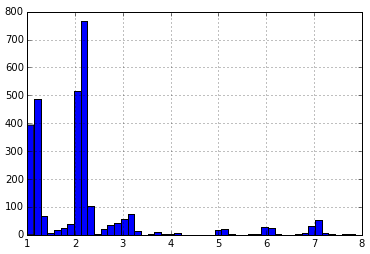
\includegraphics[width=0.9\linewidth, height=5cm]{pic/histy1.png} 
\caption{First Class}
\end{subfigure}
\begin{subfigure}[r]{0.5\textwidth}
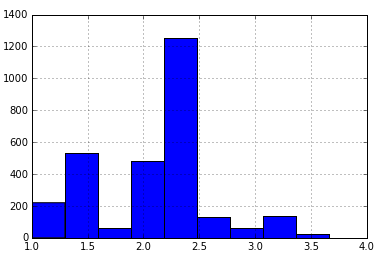
\includegraphics[width=0.9\linewidth, height=5cm]{pic/histy2.png}
\caption{Second Class}
\end{subfigure}
 
\caption{Histogram of real label and predicted label}
\label{fig:hist}
\end{figure}



\end{document}